% This file was created with tikzplotlib v0.10.1.
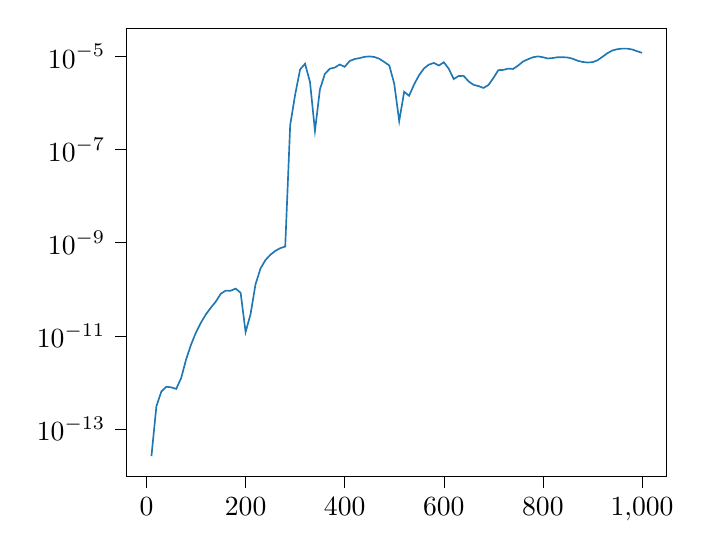
\begin{tikzpicture}

\definecolor{darkgray176}{RGB}{176,176,176}
\definecolor{steelblue31119180}{RGB}{31,119,180}

\begin{axis}[
log basis y={10},
tick align=outside,
tick pos=left,
x grid style={darkgray176},
xmin=-39.5, xmax=1049.5,
xtick style={color=black},
y grid style={darkgray176},
ymin=9.50652603798794e-15, ymax=4.01521687430453e-05,
ymode=log,
ytick style={color=black},
ytick={1e-17,1e-15,1e-13,1e-11,1e-09,1e-07,1e-05,0.001,0.1},
yticklabels={
  \(\displaystyle {10^{-17}}\),
  \(\displaystyle {10^{-15}}\),
  \(\displaystyle {10^{-13}}\),
  \(\displaystyle {10^{-11}}\),
  \(\displaystyle {10^{-9}}\),
  \(\displaystyle {10^{-7}}\),
  \(\displaystyle {10^{-5}}\),
  \(\displaystyle {10^{-3}}\),
  \(\displaystyle {10^{-1}}\)
}
]
\addplot [semithick, steelblue31119180]
table {%
10 2.60347299274599e-14
20 3.04811731410837e-13
30 6.38017416676462e-13
40 8.05272515336242e-13
50 7.81874565092266e-13
60 7.23782145328755e-13
70 1.23648313810065e-12
80 3.12141978930924e-12
90 6.46938058679325e-12
100 1.18712262242582e-11
110 1.92376392593729e-11
120 2.89670509800999e-11
130 4.02137767530064e-11
140 5.4530518989182e-11
150 8.03200284060779e-11
160 9.32434685019246e-11
170 9.29007148986472e-11
180 1.03052566480244e-10
190 8.37689362320759e-11
200 1.2031181606531e-11
210 2.90422408344426e-11
220 1.26666649391538e-10
230 2.77405709514511e-10
240 4.21934098771004e-10
250 5.48733392058409e-10
260 6.65407701161413e-10
270 7.62478635785158e-10
280 8.24771723140216e-10
290 3.34270505858436e-07
300 1.50165494919308e-06
310 5.23005855575243e-06
320 6.93951245241131e-06
330 2.80861246461372e-06
340 2.51372393955673e-07
350 1.95108579548187e-06
360 4.18930213630375e-06
370 5.42299457796658e-06
380 5.74592495915238e-06
390 6.68313980957402e-06
400 5.95694687977044e-06
410 7.93390630736412e-06
420 8.75912358315467e-06
430 9.15563077782955e-06
440 9.76221381850106e-06
450 9.9812883229411e-06
460 9.67840556008459e-06
470 8.87004661738466e-06
480 7.54454051696274e-06
490 6.37261658525956e-06
500 2.57729696102882e-06
510 4.07063187615742e-07
520 1.73542753012512e-06
530 1.42468297376075e-06
540 2.49079158387566e-06
550 3.92283099416579e-06
560 5.50329773955915e-06
570 6.66130836946e-06
580 7.21579496455738e-06
590 6.35523573404295e-06
600 7.47728776610834e-06
610 5.42760783070473e-06
620 3.25245184820688e-06
630 3.78745043075335e-06
640 3.80689885473573e-06
650 2.90563729009319e-06
660 2.44620657738337e-06
670 2.29724468735204e-06
680 2.09800116328374e-06
690 2.41991514510903e-06
700 3.41959504249895e-06
710 5.05210800540168e-06
720 5.11921492244577e-06
730 5.45816706641611e-06
740 5.36250595160187e-06
750 6.34901725327791e-06
760 7.76170568664997e-06
770 8.67975928128817e-06
780 9.55495450036259e-06
790 9.97676608501669e-06
800 9.5705870255397e-06
810 9.00975439872137e-06
820 9.20618934584921e-06
830 9.59902169543614e-06
840 9.59632225326634e-06
850 9.44533212987597e-06
860 8.88935869011037e-06
870 8.06236168350571e-06
880 7.58614191882084e-06
890 7.38342149314564e-06
900 7.48652152613577e-06
910 8.21103860248334e-06
920 9.74639645630326e-06
930 1.1665656407589e-05
940 1.33435777962612e-05
950 1.42323737731542e-05
960 1.46614786748697e-05
970 1.46395832090543e-05
980 1.40526060218998e-05
990 1.29123412733537e-05
1000 1.19141063146949e-05
};
\end{axis}

\end{tikzpicture}
